% Klassifiziert den Dokumenten-Typ
% Doku: http://exp1.fkp.physik.tu-darmstadt.de/tuddesign/
% Farben: http://www.tu-darmstadt.de/media/medien_stabsstelle_km/services/medien_cd/das_bild_der_tu_darmstadt.pdf
%  bigchapter: Chapter haben doppelte Schriftgröße
%  linedtoc: Linien im Inhaltsverzeichnis wie bei Überschriften
%  colorbacktitle: Der Dokumenten-Titel wird mir der Accentfarbe hinterlegt
\documentclass[bigchapter,colorback,accentcolor=tud4b,linedtoc,11pt]{tudreport}

% Input Dokument hat das Encoding UTF-8
\usepackage[utf8]{inputenc}
% Wichtiges Paket für Links und verlinktes Inhaltsverzeichnis
\usepackage[ngerman]{hyperref}
% Paket für Fußnoten
\usepackage[stable]{footmisc}
% Paket für amsmath (aligned mathe formeln)
\usepackage{amsmath}
% Paket für Bibliotheks-Verzeichnis, square: Verwende eckige statt runde klammern
% \usepackage[square]{natbib}
% Paket zum Plotten von Datensätzen
\usepackage{pgfplots}
\pgfkeys{%
  /pgfplots/default/.style={%
    /pgf/number format/use comma,
    legend pos=north east,
    x tick label style={/pgf/number format/1000 sep=},
    y tick label style={/pgf/number format/1000 sep=},
    width=0.9\linewidth,
    height=0.40\linewidth,
    scale only axis,
    grid=both,
    tick align=outside,
    tickpos=left,
    minor x tick num=3,
    minor y tick num=4,
    minor grid style={dotted,thin}
  }
}

% Anhänge für Original-Messdaten
\usepackage{fancyvrb}

% Verwende deutsche Bezeichner für Inhaltsverzeichnis, ... (ngerman = New German: neue Rechtschreibung)
\usepackage{ngerman}
% Deutsche Zahlen (entfernt z.B. das Leerzeichen nach einem Dezimal-Komma)
\usepackage{ziffer} 

\usepackage[verbose]{placeins}

%wegen Grafikverschiebung hinzugefügt
\usepackage{float}

%\usepackage{graphicx}
%\usepackage{caption}
\usepackage{subcaption} %Für subfigures

% PDF-Optionen
\hypersetup{%
  pdftitle={TU Darmstadt \- Physikalisches Praktikum für Fortgeschrittene},
  pdfauthor={Esra Bauer, Sören Link und Christian Hab},
  pdfsubject={Versuch 1.5},
  pdfview=FitH,
}
% Nummeriere formeln in Subsections einzeln
% Kleines makro zur assymetrischen Fehlerangabe

% Entspricht-Zeichen
\usepackage{scalerel}

\newcommand\equalhat{%
\let\savearraystretch\arraystretch
\renewcommand\arraystretch{0.3}
\begin{array}{c}
\stretchto{
    \scalerel*[\widthof{=}]{\wedge}
    {\rule{1ex}{3ex}}%
}{0.5ex}\\ 
=%
\end{array}
\let\arraystretch\savearraystretch
}
%BEGINN TITELSEITE

\title{Zeeman-Effekt}

\subtitle{Esra Bauer  \\Sören Link \\Christian Hoch}

\subsubtitle{Betreuer: Matthias Sattig \hfill Versuchsdatum: 13. April 2015}

\author{Esra Bauer, Sören Link, Christian Hoch}

%\settitlepicture{img/title.jpg}

\institution{Physikalisches Praktikum \\für Fortgeschrittene \\ Versuch 1.5}

\date{\today}
%ENDE TITELSEITE


\begin{document}
%ANFANG DOKUMENT

%Titelseite einfügen
\maketitle

%Inhaltsverzeichnis einfügen
\tableofcontents

%ANFANG INHALT

\chapter{Einleitung}

\chapter{Grundlagen}
\section{Fabry-Pérot-Interferometer}

% \begin{figure}[h] 
%   \centering
%      \includegraphics[width=0.7\textwidth]{img/...}
%   \caption{...}
%   \label{fig:...}
% \end{figure}

\section{Klassische Erklärung des Zeeman-Effekts}
\section{Quantenmechanische Kopplungen im Atom}
\subsection{LS-Kopplung}
\subsection{jj-Kopplung}
\section{Quantenmechanische Erklärungen}
\subsection{Quantenmechanische Erklärung des Zeeman-Effekts}
\subsection{Quantenmechanische Erklärung des Paschen-Back-Effekts}
\section{Auswahlregeln für Dipolübergänge}

\chapter{Durchführung}
\section{Messung von $\frac{\delta\alpha_1}{\delta\alpha_2}$}
%\begin{center}
%  \begin{tabular}{|p{2.2cm}|p{4.5cm}|p{3cm}|p{4cm}|}
%    \hline
%    Messungs-Nummer & Kristallisationstemperatur der Probe in °C & Messmethode    & Name der Messdaten-Datei \\ \hline
%    1               & 140                                        & Winkelabhängig & PET-140.0.txt \\ \hline
%    2               & 140                                        & Wanderspalt    & PET-140.ms \\ \hline
%    3               & 170                                        & Wanderspalt    & PET-170.ms \\ \hline
%    4               & 170                                        & Winkelabhängig & PET-170.0.txt \\ \hline
%    5               & 170 (Selbst getempert)                     & Winkelabhängig & PET-170-eigen.0.txt \\ \hline
%    6               & 170 (Selbst getempert)                     & Wanderspalt    & PET-170-eigen.ms \\ \hline
%    7               & 200                                        & Wanderspalt    & PET-200.ms \\ \hline
%    8               & 200                                        & Winkelabhängig & PET-200.0.txt \\ \hline
%    9               & 215                                        & Winkelabhängig & PET-215.0.txt \\ \hline
%    10              & 215                                        & Wanderspalt    & PET-215.ms \\ \hline
%	\end{tabular}
%\end{center}

\chapter{Auswertung}
\section{Überprüfung der Vorhersagen der klassischen Erklärung}

Zunächst betrachten wir den Fall des transversalen Zeemann-Effektes, also des senkrecht zur Blickrichtung ausgerichteten Magneten. In der Tat können wir, wenn der Linearpolarisator parallel zum Magnetfeld ausgerichtet ist, genau eine Spektrallinie beobachten, die bei geringfügiger Drehung des Linearpolarisators in beide Richtungen schwächer wird. Dies zeigt, dass lediglich parallel zum Magnetgeld polarisiertes Licht detektiert wird, was der Vorhersage des klassischen Modells entspricht. Wir sehen die $\pi$-Komponente, die in Richtung der z-Achse (also der Magnetfeldrichtung) schwingt und daher nicht vom Magnetfeld beeinflusst wird, also auch die gleiche Frequenz wie vorher besitzt.

Bei senkrecht zum Magnetfeld ausgerichtetem Linearpolarisator sehen wir zwei Spektrallinien im gleichen Abstand links und rechts der ursprünglichen Linie (bzw. links und rechts der $\pi$-Komponente). Daraus folgt, dass die Frequenzen dieser beiden Linien um einen bestimmten Betrag verschoben sind. Weiterhin werden die Linien schwächer, wenn man den Polarisator von der senkrechten Position wegdreht. Wir sehen hier die $\sigma^+$- und $\sigma^-$-Komponenten, die in Richtung der x-Achse schwingen, also senkrecht zum Magnetgeld polarisiert sind und um Frequenzen $\pm \omega$ von der ursprünglichen Linie abweichen.

Analog bestätigt sich das klassische Modell für den Fall des longitudinalen Zeemann-Effektes, bei dem mittels des $\frac{\lambda}{4}$-Plättchens, welches um 45$^{\circ}$ zum Linearpolarisator verdreht in den Strahlengang gebracht wird, nachgewiesen wird, dass lediglich zwei zirkular polarisierte Komponenten vorhanden sind, die entgegengesetzen Drehsinn besitzen und wiederum frequenzverschoben sind. Dies sind die $\sigma^+$- und $\sigma^-$-Komponenten, wobei die $\sigma^+$-Komponente einen mathematisch positiven Drehsinn besitzt. Dass die $\pi$-Komponente nicht sichtbar ist, erklärt sich dadurch, dass ein Hertzscher Dipol, als welchen wir das schwingende "`Ion"' betrachten, in Bewegungsrichtung nicht abstrahlt. Somit ist die klassische Vorhersage sowohl für den transversalen, als auch für den longitudinalen Zeemann-Effekt bestätigt.

\section{Überprüfung der Vorhersagen der quantenmechanischen Erklärung}

Um unsere Messdaten auswerten zu können, sind zunächst einige theoretische Vorüberlegungen notwendig. Als erstes berechnen wir die gyromagnetischen Faktoren der beteiligten Energieniveaus und tragen sie tabellarisch auf: 

\begin{center}
  \begin{tabular}{|p{2.2cm}|p{4cm}|p{2cm}|p{2cm}|}
    \hline
    Übergang & Wellenlänge in nm & ${g_J}_1$ & ${g_J}_2$ \\ \hline
    $2^3S_1~\rightarrow~2^3P_0$ & 405 & 2 & ?  \\ \hline
    $2^3S_1~\rightarrow~2^3P_1$ & 436 & 2 & $\frac{3}{2}$ \\ \hline
    $2^3S_1~\rightarrow~2^3P_2$ & 546 & 2 & $\frac{3}{2}$ \\ \hline
	\end{tabular}
\end{center}

Zeichnerisch lassen sich die erlaubten Übergänge unter Berücksichtung der Auswahlregeln in folgenden Termschemata darstellen:

\begin{figure}[H] 
  \centering
     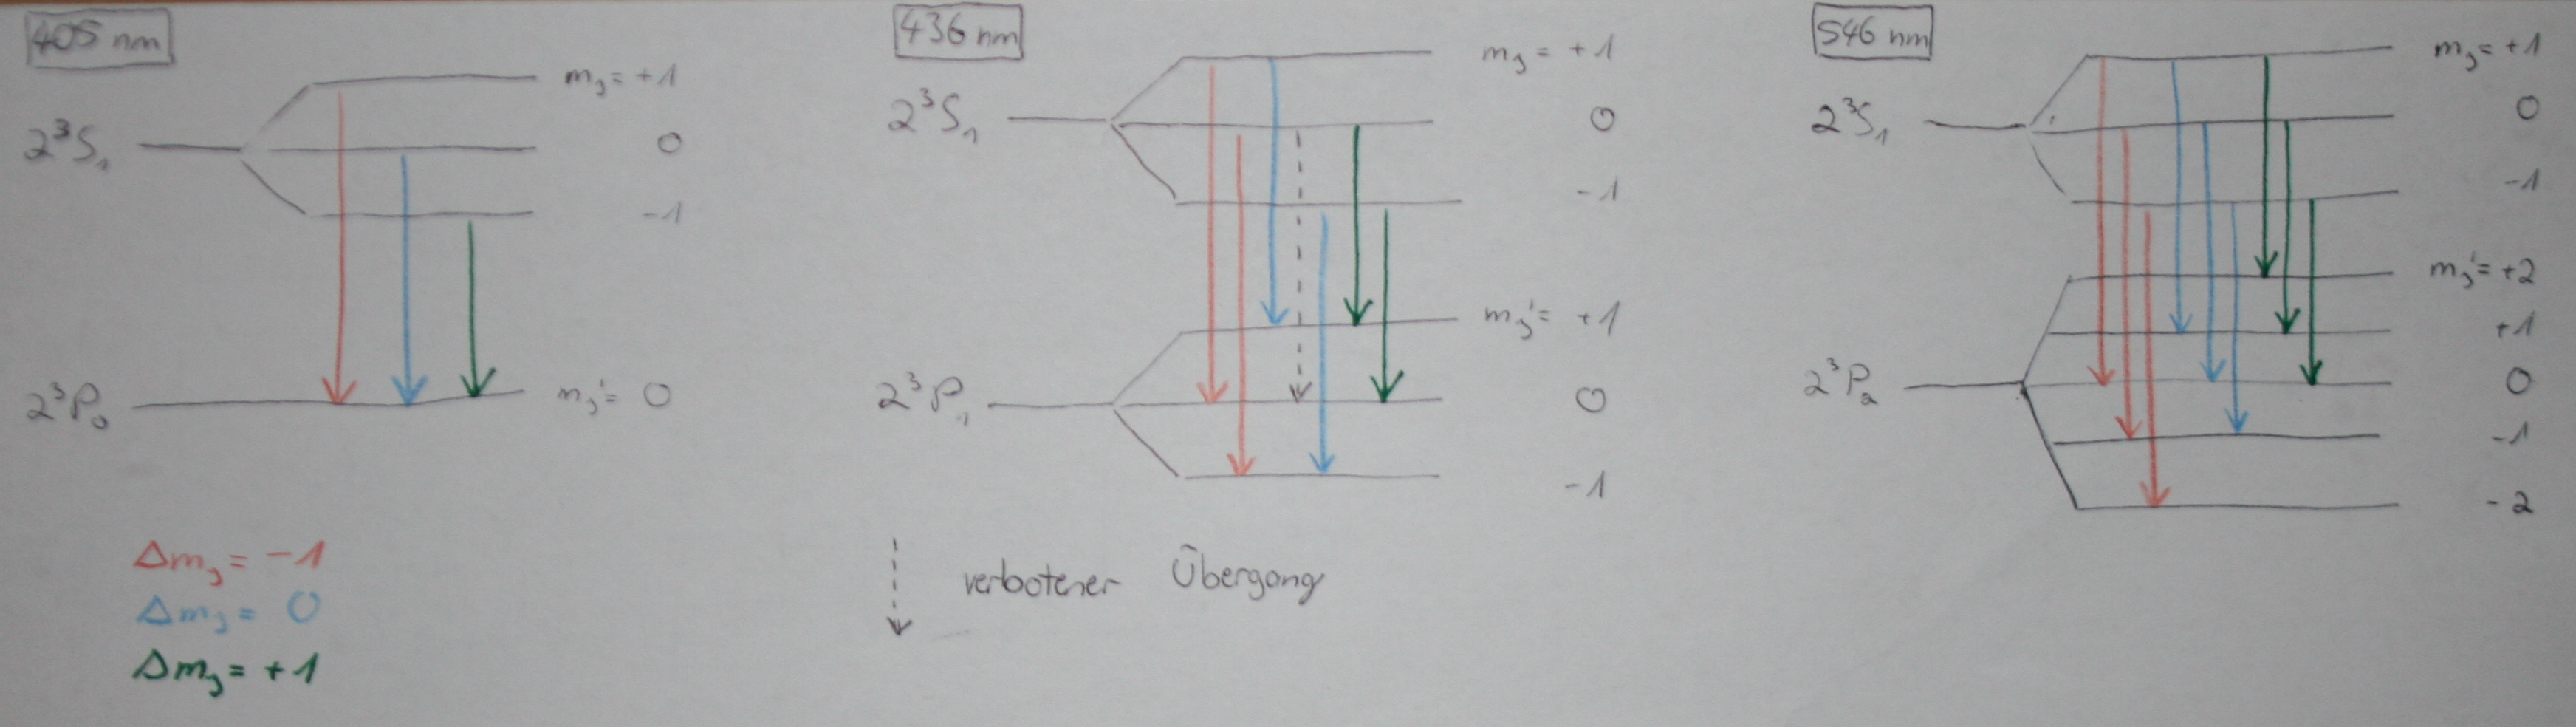
\includegraphics[width=1\textwidth]{data/Termschemata.JPG}
  \caption{Termschemata für alle drei Übergänge, oben sind jeweils die Wellenlängen eingeschrieben; verschiedene $\Delta m_J$ sind farblich gekennzeichnet. Verbotene Übergänge sind gestrichelt eingezeichnet.}
  \label{fig:Bild1}
\end{figure}

Die $g_{eff}$-Werte lassen sich leicht gemäß $g_{eff} = g_J M_J - g_J' M_J'$ berechnen und sind in folgenden Tabellen für jeden Übergang dargestellt, jeweils unterteilt in die möglichen Werte von $\Delta m_J$, also für die Änderung der magnetischen Gesamtdrehimpulsquantenzahl, die die möglichen Raumrichtungen des Drehimpulses angibt. Zunächst für 405 nm (hier ergeben sich drei Linien):

\begin{center}
  \begin{tabular}{|p{2cm}|p{2cm}|p{2cm}|p{2cm}|}
    \hline
    $\Delta m_J$ & $m_J$ & $m_J'$ & $g_{eff}$ \\ \hline
    1               & -1               & 0 &  \\ \hline
    0               & 0                & 0 &  \\ \hline
    -1              & 1                & 0 &  \\ \hline
	\end{tabular}
\end{center}

Für 436 nm sind es 6 Linien:

\begin{center}
  \begin{tabular}{|p{2cm}|p{2cm}|p{2cm}|p{2cm}|}
    \hline
    $\Delta m_J$ & $m_J$ & $m_J'$ & $g_{eff}$ \\ \hline
    1               & -1               & 0 & -2 \\ \hline
    1               & 0                & 1 & $-\frac{3}{2}$ \\ \hline
    0               & -1               & -1 & $-\frac{1}{2}$ \\ \hline
    0               & 1                & 1 & $\frac{1}{2}$ \\ \hline
   -1               & 0                & -1 & $\frac{3}{2}$ \\ \hline    
   -1               & 1                & 0 & 2 \\ \hline
    \end{tabular}
\end{center}

Für 546 nm ergeben sich sogar 9 Linien:

\begin{center}
  \begin{tabular}{|p{2cm}|p{2cm}|p{2cm}|p{2cm}|}
    \hline
    $\Delta m_J$ & $m_J$ & $m_J'$ & $g_{eff}$ \\ \hline
    1               & -1               & 0 & -2 \\ \hline
    1               & 0                & 1 & $-\frac{3}{2}$ \\ \hline
    1               & 1                & 2 & -1 \\ \hline
    0               & -1               & -1 & $-\frac{1}{2}$ \\ \hline
    0               & 0                & 0 & 0 \\ \hline
    0               & 1                & 1 & $\frac{1}{2}$ \\ \hline
    -1              & -1               & -2 & 1 \\ \hline
    -1              & 0                & -1 & $\frac{3}{2}$ \\ \hline
    -1              & 1                & 0 & 2 \\ \hline
    \end{tabular}
\end{center}

\section{Bestimmung des Bohrschen Magnetons}
%\begin{center}
%\begin{figure}[h]
% \begin{tikzpicture}
% \begin{axis}[
%     legend pos=south west,
%     title={Messereignisse in Abhängigkeit der Detektorposition},
%     xlabel=Detektorposition in µm,
%     x tick label style={/pgf/number format/1000 sep=},
%     ylabel=Messereignisse,
%     y tick label style={/pgf/number format/1000 sep=},
%     width=0.9\textwidth,
%     height= 9cm,
%     xmin=1500,
%     xmax=2500,
%     grid=both,
%     ymin=0,
%     %ymax=0.0045,
%     tick align=outside,
%     tickpos=left,
%     minor x tick num=3,
%     minor y tick num=4,
%     minor grid style={dotted,thin}
% ]
% \addplot[red, only marks, mark=x, mark size=1pt, %error bars/.cd, y dir=both, y fixed relative=0.01, x dir=both, x fixed=0.05
% ]
% table[x index={0},y index={1}] {data/beamprofile2.bp};
% %\addlegendentry{Leistung der LED auf der Photoplatte}
% \end{axis}
% \end{tikzpicture}
% \captionof{figure}{Zahl der Messereignisse über der Detektorpositon mit leeren Probenhalter, ohne beamstop und mit Messing-Strahlabsorber.}
% \end{figure}
% \end{center}
\chapter{Fazit}

%ENDE INHALT
\cleardoublepage{}
% Eintrag fürs Inhaltsverzeichnis
\newpage
\begin{thebibliography}{100}
  \bibitem{Anleitung} \url{Versuchsanleitung}
\end{thebibliography}
\end{document}
